\documentclass[serif,utf8]{beamer}
%russification
\usepackage[utf8]{inputenc}
\usepackage[russian]{babel}
%math mode
\usepackage{amssymb}
\usepackage{euscript}
\usepackage{amsmath}
\usepackage{amstext}
\usepackage{textcomp}
\usepackage{graphicx}
\usepackage{fancybox}
\usepackage{wrapfig}
\usepackage{multicol}
\usepackage{multirow}
%\usepackage[final]{graphicx}
\graphicspath{{image/}}

\usepackage{floatflt}
%\usepackage{pst-plot}
%theme
\usetheme{Copenhagen}

\usecolortheme{seahorse}

\setbeamersize{text margin left = 1.0 cm}
\setbeamersize{text margin right = 1.0 cm}

\setbeamertemplate{caption}[numbered]


\newtheorem{mydef}{Определение}

\begin{document}

%\setbeamercolor{block body}{BG=green}

\institute{Московский Государственный Университет им. М.В. Ломоносова \\ %
	факультет Вычислительной математики и кибернетики \\ %
	кафедра Математических Методов Прогнозирования }
\title[Предсказание затрат]{Предсказание затрат}
\author[Трубицын Ю. А.]{Трубицын Юрий Алексеевич}
\date{Москва, 2017}


\begin{frame}
\maketitle
\end{frame}


\begin{frame}
\frametitle{Постановка задачи}
\begin{itemize}
\item \textbf{Дано:} данные о 110000 клиентах некоторого магазина. Данные имеют следующий формат:
	\begin{itemize}
	\item Поле \textit{<<id>>} - идентификатор клиента;
	\item Поле \textit{<<date>>} - дата покупки;
	\item Поле \textit{<<sum>>} - сумма покупки.
	\end{itemize}
\item \textbf{Выход:} для каждого клиента вывести сумму его первой покупки
на следующей неделе. Если клиент ничего не купит в течении недели, то вернуть ноль.
\item \textbf{Метрика:} accuracy.
\end{itemize}
\end{frame}

\begin{frame}
\frametitle{Наблюдения}
\begin{figure}[h!]
   \centering
   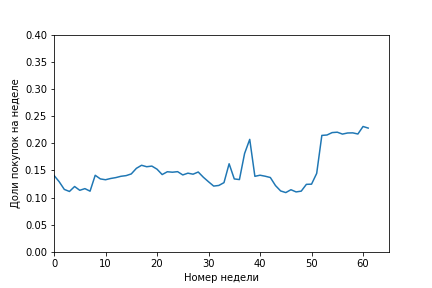
\includegraphics[width=0.7\linewidth]{PartsZero.png}
\end{figure}
Указана доля <<покупок>> на сумму 0 за каждую неделю. Но это мало информативно.
\end{frame}

\begin{frame}
\frametitle{Наблюдения}
\begin{figure}[h!]
   \centering
   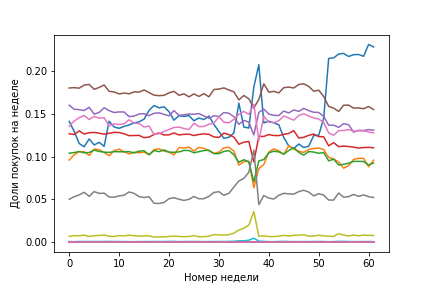
\includegraphics[width=0.7\linewidth]{PartsBad.png}
\end{figure}
Указаны доли всех первых сумм покупок по неделям. Можно <<почистить>> выборку.
\end{frame}

\begin{frame}
\frametitle{Наблюдения}
\begin{figure}[h!]
   \centering
   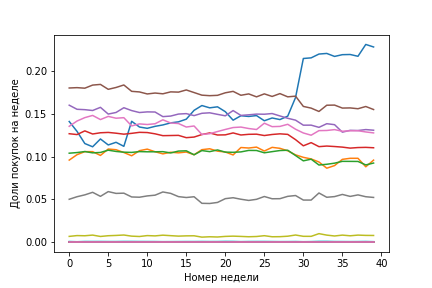
\includegraphics[width=0.7\linewidth]{PartsGood.png}
\end{figure}
Выглядит уже более стабильно.
\end{frame}

\begin{frame}
\frametitle{Идея}
Что предпринималось:
\begin{itemize}
\item \textbf{Способ 1:} попытка спрогнозировать долю каждой суммы на следующую неделю и <<расфасовать>> клиентов по суммам, согласно распределению первых сумм за неделю каждого клиента;
\item \textbf{Способ 2:} Использовать весовую схему с весами, равными степени номера недели.
\end{itemize}
\end{frame}

\begin{frame}
\frametitle{Способ борьбы с нулевыми покупками}
На графиках хорошо видно что в конце выборки многие клиенты перестали ходить 
в данный магазин. Способ борьбы - сумма для клиентов, которые не ходили 
больше некоторого порога автоматически выставляется нулем.

\end{frame}

\begin{frame}
\frametitle{Способ тестирования}
Способ тестирования достаточно прост
\begin{itemize}
\item <<Отсекаем>> от выборки последнюю неделю;
\item Пытаемся предсказать по <<усеченной>> выборке;
\item Сравниваем предсказание с точным ответом и выдаем долю верно предсказанных ответов. 
\end{itemize}
\end{frame}

\begin{frame}
\frametitle{Результаты}
\begin{enumerate}
\item \textbf{Способ 1 (восстановление долей):}
	\begin{itemize}
	\item Тестирование: 0.38664
	\item Leaderboard: 0.39000
	\end{itemize}
\item \textbf{Способ 2 (весовая схема):}
	\begin{itemize}
	\item Тестирование: 0.39287
	\item Leaderboard: 0.39715
	\end{itemize}
\end{enumerate}
\end{frame}

%\begin{frame}
%\frametitle{Что за данные?}

%\end{frame}

\end{document}